\documentclass[11pt, a4paper]{report}
\usepackage[utf8]{inputenc}

\usepackage{listings}
\usepackage[framed,numbered,autolinebreaks,useliterate]{mcode}

\usepackage[margin=1in]{geometry}
\usepackage{graphicx}
\usepackage{amsmath}
\usepackage{amsfonts}
\usepackage{caption}
\usepackage{float}
\usepackage[hyphens,spaces,obeyspaces]{url}
\usepackage{hyperref}
\usepackage{appendix}
\usepackage{chngcntr}
\usepackage{etoolbox}
\usepackage{lipsum}
\usepackage{tikz}
\graphicspath{ {images/} }
\setlength\parindent{0pt}


\newcommand{\p}{\partial}
\newcommand{\mth}[1]{
  \begin{align*}
    #1
  \end{align*}
}


\usetikzlibrary{shapes.geometric, arrows}

\newcommand{\newappendix}{%
  \refstepcounter{chapter}\chapter*{Appendix \thechapter}%
  \addcontentsline{toc}{chapter}{Appendix \thechapter}%
}
\tikzstyle{block} = [rectangle, rounded corners, minimum width=3cm, minimum height=1cm,text centered, draw=black, fill=white!30]
\tikzstyle{startstop} = [rectangle, rounded corners, minimum width=3cm, minimum height=1cm,text centered, draw=black, fill=red!30]
\tikzstyle{io} = [trapezium, trapezium left angle=70, trapezium right angle=110, minimum width=3cm, minimum height=1cm, text centered, draw=black, fill=blue!30]
\tikzstyle{process} = [rectangle, minimum width=3cm, minimum height=1cm, text centered, draw=black, fill=orange!30]
\tikzstyle{decision} = [diamond, minimum width=3cm, minimum height=1cm, text centered, draw=black, fill=green!30]
\tikzstyle{arrow} = [thick,->,>=stealth]

\begin{document}

\begin{center}
  \Huge Floppy Drive Orchestra \\
  \huge University of Colorado Boulder \\
  \Large Independent Study 2017\\
  
  \vspace{6in}
    \huge Jeffery Lim \\
    \huge Jeffery.Lim@colorado.edu\\
    \Large Under supervision of Dr. Shalom Ruben \\~\\~\\
\end{center}

\tableofcontents

\chapter{Introduction}

The goal of this independent study is to build a working implementation of the floppy drive orchestra and understand each process that allows it to produce music. Floppy drives are hardware devices that were invented in 1967 for storing information. Floppy drives are now ancient in comparison to current storage devices, so there are no reason to use them in modern computers. People have found alternative uses for them. The floppy drive has a stepper motor that makes an audible sound each time it moves. Since sound is the basis of music, floppy drives can produce music. \\

To properly understand the orchestra, the floppy drive physical characteristics are needed. Characteristics like the physical limitations of the read/write head and what range of frequencies can the stepper motor handle give insight to how sound is produced from the floppy drives. The necessary hardware to enable the floppy drive orchestra is simple with minimal work. The software that goes into running the orchestra, however, is the most complicated part. It required understanding music file format and understanding the controls necessary to operate several floppy drive in sync. \\


\chapter{Floppy Drive Characteristics}

The tests conducted to understand the characteristics were done with a single floppy drive. Floppy drives come in three sizes: 8 in., 5.25 in., and 3.5 in. All different sizes give different characteristics, but for this implementation, the more modern 3.5 in. floppy drives were used. The five characteristics to be explored are the pin outs, power consumption, stepper motor movements, stepper motor bandwidth, and frequency.

\begin{figure}[H]
\hspace*{-2cm}    
    \centering
    \includegraphics[width=.5\textwidth]{floppydrive_sizes.jpg}
    \caption{Floppy Drive of All Sizes}
    \label{fig:sizes}
\end{figure}

\section{Floppy Pinout}

The floppy drive pins are shown in Figure \ref{fig:pinOut}. All the bottom row pins are odd numbered while the top row pins are even numbered. The bottom row pins are all grounded while the top row pins are 5V. Each pin has a different functionality when it is grounded. Each function is shown in Figure \ref{fig:pinNames}. 

\begin{figure}[H]
\hspace*{-2cm}    
    \centering
    \includegraphics[width=.75\textwidth]{floppy_pinout.jpg}
    \caption{Floppy Drive Pinout}
    \label{fig:pinOut}
\end{figure}

\begin{figure}[H]
\hspace*{-2cm}    
    \centering
    \includegraphics[width=.75\textwidth]{pinNames.png}
    \caption{Floppy Drive Pin Names}
    \label{fig:pinNames}
\end{figure}
 
The majority of the pins are used for memory management purposes. The only necessary pins to drive the floppy drive are pin numbers 12 or 14, 18, and 20.\\

Pins 12 and 14 are respectively known as drive select B and A. These pins are enable pins for the floppy drives and without connecting these pins to ground, the drive will not operate. Each drive usually has a different drive letter. In order to see which drive letter it is, connect the power (See Section \ref{POWER} for more details on powering the floppy drives) to the floppy drive and connect pin 12 or 14 to any of the ground pins. The LED in the front of the drive should turn on for one them. \\

Pin 18 is the direction pin. The direction pin determines which direction the read/write head is moving. When the direction pin is grounded, the drive will move away from the pins and vice versa when the pin is held high. \\

Pin 20 is the step pin. This pin drives the stepper motor. Every time the voltage at the pin transitions from low to high, the stepper motor will go forward one tick.\\

Figure \ref{fig:pins} highlights the locations of the pins for operating a single floppy drive. All the drives tested were B drives.

\begin{figure}[H]
\hspace*{-2cm}    
    \centering
    \includegraphics[width=.75\textwidth]{floppy_pinoutV1.jpg}
    \caption{Floppy Drive Necessary Pins}
    \label{fig:pins}
\end{figure}

\section{Power}\label{POWER}

The floppy drive is powered by a mini Molex cable. A mini Molex cable, as seen in Figure \ref{fig:miniMolex}, has one red, one yellow, and two black wires. The two black wires are grounds, where the red line is 5V and the yellow is 12V. Older generation floppy drives used both the 5V and 12V, where the 12V was used to power the stepper motor. Modern floppy drives no longer use the 12V and use the 5V for everything. This means there is no need for any regulation, and as long as the power supply provides enough current, 5V is sufficient. 

\begin{figure}[H]
\hspace*{-2cm}    
    \centering
    \includegraphics[width=.4\textwidth]{miniMolex.jpg}
    \caption{Floppy Drive Power Pinout}
    \label{fig:miniMolex}
\end{figure}

The power consumption was measured by using jumper cables to connect the floppy drives to a power supply with an ammeter to measure the current. Pin 12 was grounded to enable drive B and a function generator was connected to pin 20. Without turning on the function generator, the idle current is 50 mA. To test when active, pin 18 was connected to ground and disconnected in order to allow for the read/write head to continue moving. The function generator was swept to multiple frequencies to see if the input frequency changed the power consumption. When active, the floppy drive pulls 400 mA regardless of the frequency of the input. Each floppy drive that is added to the system will require an additional 400 mA to the power budget. \\

\section{Stepper Motor Movement}

\begin{figure}[H]
\hspace*{-2cm}    
    \centering
    \includegraphics[width=.5\textwidth]{floppydrive_coveroff.jpg}
    \caption{Floppy Drive With Top Off}
    \label{fig:coveroff}
\end{figure}

The floppy drive read/write head has a physical limit to how far it can go. To determine this value, a 1 Hz square wave is sent through to the floppy drive's step pin (pin 20). The drive enable pin (pin 12) is grounded, and the pin 18 is set to ground. The number of ticks is manually recorded by counting the number of audible ticks that can be heard, with the last value is when the read/write head does not move. This can be run multiple times by simply disconnected or connecting the direction pin (pin 18). \\

The total number of ticks a 3.5 in. drive can go is 80, meaning the step pin (pin 20) needs to be toggled high 80 times before the drive reaches the limit. This means there needs to be a transition of high to low 80 times, or a total of 160 voltage transitions. \\

One interesting result from this experiment was that each floppy drive has a different behavior when the read/write head reached its limit. Some floppy drives will try to move the head further, which results in the head to continuously tick. Other floppy drives will not make any noise and will stay in place.

\section{Stepper Motor Bandwidth}

Since the music will be played through the read/write head, the bandwidth of the stepper motor will be a large limiting factor. For the test, a square wave from a waveform generator is connected to the step pin (pin 20), and the direction pin is connected to ground and disconnected in order to allow the read/write head to switch direction. \\

The waveform generator is swept from 1 Hz up until the read/write head is no longer moving. The drive was able to handle up to 400 Hz, but afterwards, it was no longer consistent in terms of the speed of the drive. This test is ran again when the software was fully written. This made a significant difference because the motor was able to run at a much higher input frequency. It is not quite clear why the floppy drive was able to run at higher speeds with the software. It is possible that the cable used in the experiment with the function generator may have caused the signals to deteriorate once they reached the floppy drive pins. \\ 

This limit considerably restricts what the drive can play, and higher notes will need to be addressed. However, so far, there is an assumption that the audible range contains the input frequency given to the stepper motor. In the next section, audio files of the floppy drives at each frequency are recorded and transformed. \\

\section{Frequency}

Although the floppy drive was unable to run past 400 Hz using the function generator, it is also important to take a look at the actual audio produced from the floppy drive. The experiment is to understand whether or not the note being played from the floppy drive has the same frequency as what is being pushed through the floppy. \\

Because of scheduling conflicts, an analysis of the recordings were not done. The test to be done will be discussed instead. \\

The first test is to be conducted in an anechoic chamber so that any stray sounds is absorbed by the room. The recording can be done all at once, however, after the recording, the audio file needs to be clipped appropriately so each note is analyzed separately. The test plays the same note at different octaves. If the note played is C, then the first note to be played would be C-1, followed by C0, C1, etc. The last note played would be C9. A Fast Fourier Transform of each note will reveal whether or not the audio file's peak frequency is the same as the notes actual frequency. This relationship between the note and the frequency can be found in Figure \ref{fig:Piano} and Table \ref{fig:note2freq}. \\


From observations, depending on the direction that the read/write head is going, it makes a different sound. This means that if a note is being held for a long time, there will actually be an audible difference as the head goes back and forth. What is not obvious, however, is how different the two are. The second test is to figure out how different the sounds are. The test is similar to the previous one, however, special care must be taken so that the initial direction of the head is known. Once the recordings are finished, the audio files need to be clipped to separate the recordings of each direction. \\



\chapter{Hardware}

The Arduino provides a lot of flexibility with the shields that interface with it. The shield used in this project provided the necessary power and connections to the floppy drive. The parts and components used can be found in the Bill of Materials found in Appendix \ref{fig:BOM}.

\section{Power}

As discussed in the previous chapter on floppy drive power characteristics, since each floppy drive draws a maximum of 400 mA, the total power consumption required will simply be the number of floppy drives multiplied by 400 mA. For 8 floppy drives, the total power consumption from the floppy drive system would be around 3200 mA, or 3.2 A. This means the power supply would need to be at least 4 A to take into consideration of the Arduino power consumption. This extra 800 mA would be plenty of enough to power the Arduino and run very extensive code. \\

The power is supplied from a 5V 4A power supply. This is directly connected into a power terminal. The original power input that comes with the Arduino cannot supply enough current because the regulator limits the current output. Instead, another power terminal needs to be soldered onto the shield. The grounds should be connected to the Arduino and the 5V should be connected to 5V on the Arduino. \\
  
\section{Cables}
All the wires bought were from Pololu, which can be found in the BOM at Table \ref{fig:BOM}. \\

To build the wires, pre-crimped female terminal wires were used. For the power cord to the floppy drives, a red and black wire to connected to a 1 x 2 pin housing. \\

The cables for the pins on the floppy drive consist of a 2 x 10 housing on the floppy drive side. This housing would be connected to the far left side of the floppy drive pins. The only pins connected are the same as seen in Figure \ref{fig:pins}. Pins 11 and 12 are connected to black pre-crimped wires. Pin 18 is connected to a blue pre-crimped wire and pin 20 is connected to a purple pre-crimped wire. \\

\begin{figure}[H]
\hspace*{-2cm}    
    \centering
    \includegraphics[width=.5\textwidth]{floppy_wire.jpg}
    \caption{Data Cable on Floppy Side}
    \label{fig:floppywire}
\end{figure}


On the other end of the data cable is a 2 x 2 pin housing. The order is significant and must be kept track of because the software needs to know which pins are direction and step. The two black wires can be connected to any pins, as long as they are on the same side. The blue and purple pin need to be in the following order: blue on the left, and purple on the right. This needs to be consistent because all of the direction pins are on even numbered pins and the step pins are on odd numbered pins. If one wanted to flip the pins, they would need to change the software to match it. \\

\begin{figure}[H]
\hspace*{-2cm}    
    \centering
    \includegraphics[width=.5\textwidth]{arduino_wire.jpg}
    \caption{Data Cable on the Arduino Side}
    \label{fig:arduinowire}
\end{figure}


\section{Schematic}

To incorporate the necessary circuitry to power the floppy drives and organize the data pins, an Arduino shield makes it extremely flexible. The shield purchased can be found in Table \ref{fig:BOM}. There are many ways of setting the shield up, however, this is the way that was done. 

With the shield, solder on all the components that come with the shield. Once finished, then following the layout of the shield as seen in Figure \ref{fig:TOP}.

\begin{figure}[H]
\hspace*{-2cm}    
    \centering
    \includegraphics[width=.5\textwidth]{TOP.jpg}
    \caption{Top of the Shield}
    \label{fig:TOP}
\end{figure}

On the left of Figure \ref{fig:TOP} is the power terminal. This is where the 5V power supply would be plugged into. \\

In the center of the shield, there is a row of connections that are 5V and ground. Male headers are soldered to the center so they can be connected to the cable that power the floppy drives. \\

For the floppy drive pins, two rows of male headers are placed along the analog pins and the digital pins. The inner row of headers are all connected to ground. These are the headers which the drive select pins should be connected to. The other row of headers are the step and direction pin. \\

In Figure \ref{fig:TOP1} and \ref{fig:TOP2}, the yellow wires are connecting the direction and step pins to the Arduino pins. \\


\begin{figure}[H]
\hspace*{-2cm}    
    \centering
    \includegraphics[width=.5\textwidth]{TOP1.jpg}
    \caption{Top of the Shield}
    \label{fig:TOP1}
\end{figure}

\begin{figure}[H]
\hspace*{-2cm}    
    \centering
    \includegraphics[width=.5\textwidth]{TOP2.jpg}
    \caption{Top of the Shield}
    \label{fig:TOP2}
\end{figure}


The schematic of the board is shown below. 

\begin{figure}[H]
\hspace*{-2cm}    
    \centering
    \includegraphics[width=\textwidth]{schematic.png}
    \caption{Schematic}
    \label{fig:SCHEMATIC}
\end{figure}

The current iteration of the board has all step pins on the odd numbered pins while the direction pins are on the even numbered pins. This can be changed by changing the wiring, as long as it is clear which pin on the Arduino is talking to the direction and step pins.

\chapter{MIDI Files}

MIDI, or Musical Instrument Digital Interface, is a standard that has its own protocols, interface, and connectors. It allows a single file to contain multiple tracks for several instruments in its own channel. This allows a MIDI file to play several instruments at once, up to a maximum of 16 instruments. This advantage of the MIDI file allows multiple floppy drives to be played at once, like how a MIDI file would normally send notes to several instruments. The MIDI file is the main reason why the floppy drive orchestra is possible. Without it, the only way to replicate notes is by manually playing them. 

\section{MIDI Notes}

The MIDI interface has notes that are mapped to specific piano keys at their respected frequencies. Each note is represented by a byte, or 8 bits. It only uses the lower 7 bits, so the note values go from 0 to 127. In Figure \ref{fig:Piano}, the respected MIDI note number has an associated piano key, since the MIDI note is based on music pitch. 

\begin{figure}[H]
\hspace*{-2cm}    
    \centering
    \includegraphics[width=.75\textwidth]{midi_notechart.jpg}
    \caption{MIDI Note Number to Piano Key}
    \label{fig:Piano}
\end{figure}

In Table \ref{fig:note2freq}, the actual frequency of the MIDI note number is displayed in hertz. Because the floppy drive maximum bandwidth is about 400 Hz, notes 0 to 67, or at least half of the range, can be played.

\captionof{table}{MIDI Note to Frequency}\label{fig:note2freq}
\begin{center}
 \begin{tabular}{|c|c||c|c||c|c||c|c|} 
 \hline
 MIDI Note& Hz & MIDI Note& Hz & MIDI Note& Hz & MIDI Note&Hz\\
 \hline
 0 & 8.18 & 32 & 51.91& 64 & 329.63 & 96 & 2093.00 \\
 \hline
1 & 8.66 & 33 & 55.00& 65 & 349.23 & 97 & 2217.46 \\
 \hline
2 & 9.18 & 34 & 58.27& 66 & 369.99 & 98 & 2349.32 \\
 \hline
3 & 9.72 & 35 & 61.74& 67 & 392.00 & 99 & 2489.02 \\
 \hline
4 & 10.30 & 36 & 65.41& 68 & 415.30 & 100 & 2637.02 \\
 \hline
5 & 10.91 & 37 & 69.30& 69 & 440.00 & 101 & 2793.83 \\
 \hline
6 & 11.56 & 38 & 73.42& 70 & 466.16 & 102 & 2959.96 \\
 \hline
7 & 12.25 & 39 & 77.78& 71 & 493.88 & 103 & 3135.96 \\
 \hline
8 & 12.98 & 40 & 82.41& 72 & 523.25 & 104 & 3322.44 \\
 \hline
9 & 13.75 & 41 & 87.31& 73 & 554.37 & 105 & 3520.00 \\
 \hline
10 & 14.57 & 42 & 92.50& 74 & 587.33 & 106 & 3729.31 \\
 \hline
11 & 15.43 & 43 & 98.00& 75 & 622.25 & 107 & 3951.07 \\
 \hline
12 & 16.35 & 44 & 103.83& 76 & 659.26 & 108 & 4186.01 \\
 \hline
13 & 17.32 & 45 & 110.00& 77 & 698.46 & 109 & 4434.92 \\
 \hline
14 & 18.35 & 46 & 116.54& 78 & 739.99 & 110 & 4698.64 \\
 \hline
15 & 19.45 & 47 & 123.47& 79 & 783.99 & 111 & 4978.03 \\
 \hline
16 & 20.60 & 48 & 130.81& 80 & 830.61 & 112 & 5274.04 \\
 \hline
17 & 21.83 & 49 & 138.59& 81 & 880.00 & 113 & 5587.65 \\
 \hline
18 & 23.12 & 50 & 146.83& 82 & 932.33 & 114 & 5919.91 \\
 \hline
19 & 24.50 & 51 & 155.56& 83 & 987.77 & 115 & 6271.93 \\
 \hline
20 & 25.96 & 52 & 164.81& 84 & 1046.50 & 116 & 6644.88 \\
 \hline
21 & 27.50 & 53 & 174.61& 85 & 1108.73 & 117 & 7040.00 \\
 \hline
22 & 29.14 & 54 & 185.00& 86 & 1174.66 & 118 & 7458.62 \\
 \hline
23 & 30.87 & 55 & 196.00& 87 & 1244.51 & 119 & 7902.13 \\
 \hline
24 & 32.70 & 56 & 207.65& 88 & 1318.51 & 120 & 8372.02 \\
 \hline
25 & 34.65 & 57 & 220.00& 89 & 1396.91 & 121 & 8869.84 \\
 \hline
26 & 36.71 & 58 & 233.08& 90 & 1479.98 & 122 & 9397.27 \\
 \hline
27 & 38.89 & 59 & 246.94& 91 & 1567.98 & 123 & 9956.06 \\
 \hline
28 & 41.20 & 60 & 261.63& 92 & 1661.22 & 124 & 10548.08 \\
 \hline
29 & 43.65 & 61 & 277.18& 93 & 1760.00 & 125 & 11175.30 \\
 \hline
30 & 46.25 & 62 & 293.66& 94 & 1864.66 & 126 & 11839.82 \\
 \hline
31 & 49.00 & 63 & 311.13& 95 & 1975.53 & 127 &  12543.85 \\
 \hline
 \end{tabular}
\end{center}


\section{MIDI} \label{MIDIMESSAGE}

MIDI data is sent serially, meaning the data is sent one bit at a time. As a result, the Arduino reads the data from a serial port. In order to know how to design the software to accept and understand the MIDI data, the messages need to be understood. MIDI files are separated into two parts: a header chunk and a track chunk. The header chunk gives information about the song, such as the number of tracks it has, the beats per quarter note of the song, and other information. The track chunk contains the notes of the song.

\subsection{Header Chunk}

\captionof{table}{Header Chunk}\label{fig:header}
\begin{center}
 \begin{tabular}{||c | c | c | c | c||} 
 \hline
  \multicolumn{5}{|c|}{Header Chunk} \\ 
 \hline
  \multicolumn{3}{|c|}{Chunk Type}  & Length & Data \\
 \hline
  ASCII (4 Bytes) & Length of Data(4 Bytes)  & Format (16 bits) & Tracks (16 bits) & Division (16 bits) \\
 
 \hline
\end{tabular}
\end{center}


The first 4 bytes of any chunk is an ASCII representation of what type of chunk it is. This is always MThd for the header chunk. The next 4 bytes is the length of the data section. The data section is usually always 6 bytes. The next 16 bits i the MIDI format. MIDI files comes in three formats: Format 0, Format 1, and Format 2. \\

\begin{itemize}
  \item Format 0 is a single track format, where there is only one track or one instrument
  \item Format 1 has multiple tracks, each to be played simultaneously
  \item Format 2 has multiple tracks, each to be played independently
\end{itemize}

 After the format, The next 16 bits are the number of tracks. The last 16 bits are the time divisions. The value dictates the resolution of the MIDI file. In other words, it gives the relation between a MIDI tick in a song and time. 

\subsection{Track Chunk}

The track chunk starts out the same as the header chunk. The first 4 bytes are the ASCII representation and is always MTrk. It then gives the length of data of the data section. This value is sometimes accurate, but it is commonly recognized in the community as not usually accurate. The last section is the data. This contains the delta times and events which make up the notes that are to be played. 

\captionof{table}{Track Chunk}\label{fig:track}
\begin{center}
 \begin{tabular}{||c | c | c||} 
 \hline
  \multicolumn{3}{|c|}{Track Chunk} \\ 
 \hline
  Chunk Type & Length & Data \\
 \hline
  ASCII (4 Bytes) & Length of Data(32 bits)  &  Delta Time and Events \\
 
 \hline
\end{tabular}
\end{center}


\subsection{MIDI Message}

The events that the track chunk contains are the MIDI messages that contain the song content. Each message comes in 3 bytes. The first byte is a status byte that contains a command and channel. There are several commands, but for the floppy drive orchestra, there are only two significant commands: note on and note off. The channel bits are the MIDI channels that the message is being sent to. \\

The last two bytes are note and velocity The velocity represents the loudness of the note, where zero represents no sound. Since the floppy drive produces a constant sound, the velocity bit can be ignored. \\

\captionof{table}{MIDI Message}\label{fig:midimessage}
\begin{center}
 \begin{tabular}{||c | c | c | c | c||} 
 \hline
  \multicolumn{5}{|c|}{MIDI Message} \\ 
 \hline\hline
  \multicolumn{3}{|c|}{Status}  & Data & Data \\
 \hline
  \multicolumn{2}{|c|} {Command (4 bits)} & Channel(4 bits)  & Note (8 bits) & Velocity (8 bits) \\
 \hline
  Note On & 1001 & nnnn  & 0xxxxxxx & 0vvvvvvv \\
 \hline  
  Note Off  & 1000 & nnnn  & 0xxxxxxx & 0vvvvvvv \\
 \hline
\end{tabular}
\end{center}

\subsection{Delta Time}

Delta time is the number of ticks needed until the next event. This is a crucial part of the data stream because it lets the instrument or player know that there needs to be waiting until the next note plays. This part is not important to running the floppy drive orchestra from the computer because the player will handle the ticks. \\

In the case that the Arduino is acting as the player, the delta time message is a very complicated process. Each tick is of a variable length. If the value is greater than or equal to 0x80, the top bit is cut off, and it is concatenated to the next delta message. This continues until the next value is not greater than or equal to 0x80.

\section{Extra Sources}

There are a lot more details to the MIDI files and how it is formated. Here are some more references that provide more detail. \\


\begin{center}
 \begin{tabular}{|c | c |} 
 \hline
  Topic & URL \\
  \hline
  MIDI Messages & \cite{MIDIMessage} \\
  \hline
  MIDI file outline & \cite{MIDIFileOutline} \\ 

  \hline
   MIDI file format Standard &  \cite{MIDIFormat} \\
   \hline
   MIDI Tutorial & \cite{MIDITutorial}\\ 
   \hline
\end{tabular}
\end{center}

\chapter{Software}

In order to run the software, there needs to be information to be sent from a computer to the Arduino. The data flow path of the driver is as following. 

\begin{center}
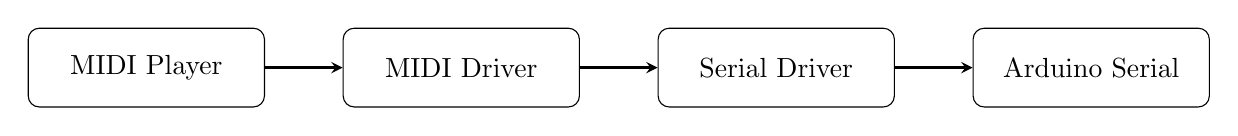
\begin{tikzpicture}[node distance=2cm]

\node (block) [block] {MIDI Player};
\node (block1) [block, right of=block, xshift=2cm] {MIDI Driver};
\node (block2) [block, right of=block1, xshift=2cm] {Serial Driver};
\node (block3) [block, right of=block2, xshift=2cm] {Arduino Serial};

\draw [arrow] (block) -- (block1);
\draw [arrow] (block1) -- (block2);
\draw [arrow] (block2) -- (block3);

\end{tikzpicture}
\end{center}

The MIDI player handles all the MIDI file format and essentially plays the music. The MIDI driver takes the information from the MIDI player and converts it into serial data. The serial data is sent over USB to the Arduino. \\

The floppy drive orchestra currently only works on Linux. The limiting factor of the orchestra is the inability to find the proper music player that will work with MIDI to Serial drivers. If the correct player can be found, this system will be able to work on Windows and Mac.

\section{MIDI to Serial Driver}

The MIDI to serial driver is a key player in getting music to play on the floppy drives. The driver turns the MIDI outputs from the player, into data that is transmitted using serial. The driver used for this project was Hairless MIDI to Serial Bridge, found at \cite{HairlessMIDI}. \\

This project has platforms for all three operating systems and has a GUI that is easy to interface with as evident in Figure \ref{fig:hairless}. The Serial to MIDI Bridge On turns the driver on or off, being necessary with reprogramming the Arduino since the Arduino requires the serial port to be programmed. The Serial Port drop down menu will have the name of the Arduino or the COM port being used by the Arduino. The MIDI In drop down menu is where the MIDI player or piano should be located. \\

\begin{figure}[H]
\hspace*{-2cm}    
    \centering
    \includegraphics[width=.75\textwidth]{MIDISerial_Bridge.png}
    \caption{Hairless MIDISerial}
    \label{fig:hairless}
\end{figure} 

Another alternative in the case that Hairless MIDI does not work is called ttymidi, found at \cite{ttymidi}. Since ttymidi does not have a GUI, it is much more difficult to work with it. It also has some bugs in the code, however, will work on most Linux platforms. Further information on how to install and run ttymidi will be explained later on. 

\section{Virtual Keyboard}

There is a program called VMPK or Virtual MIDI Piano Keyboard that sends MIDI file based on the note played \cite{VMPK}. This is a great way of testing the MIDI parser on the Arduino and testing the floppy drive's responsiveness to different notes. It will work on Linux or Mac.  

The only necessary step is to go to EDIT -$>$ MIDI Connections and make sure that Enable MIDI input is selected as following:

\begin{figure}[H]
\hspace*{-2cm}    
    \centering
    \includegraphics[width=.75\textwidth]{HairlessSetup.png}
    \caption{Hairess MIDI Setup}
    \label{fig:hairlesssetup}
\end{figure} 

Once it is enabled, Hairless MIDI should show an option to set MIDI IN to VMPK. This will route the MIDI notes played from the piano to the Arduino. \\

An alternative keyboard is called vkeybd. It can be installed with apt-get.

\begin{lstlisting}[language=bash]
  $ sudo apt-get install vkeybd
\end{lstlisting}

The keyboard is similar to VMPK but has a simple GUI. 

\begin{figure}[H]
\hspace*{-2cm}    
    \centering
    \includegraphics[width=.75\textwidth]{vkeybd.png}
    \caption{Virtual Keyboard}
    \label{fig:vkeybd}
\end{figure} 

It can be run by using the command:

\begin{lstlisting}[language=bash]
  $ vkeybd
\end{lstlisting}

In order to interface it with Hairless MIDI, the MIDI IN will have a drop down option for vkeybd, similar to VMPK. \\

If using ttymidi, refer to the instructions found in section \ref{ttymidiSECTION}.

\section{MIDI Player}

The MIDI player is just like any audio player, with the ability to parse through the MIDI file format. There are specifications that must be met in order to use a MIDI player with the serial driver. The Hairless MIDI to Serial Bridge website, \cite{HairlessMIDI} does a good job of explaining further what needs to be done in order to work with MIDI players, but does not provide any programs that work with them. The MIDI player does some back-work for the Arduino: it handles the header and the delta time ticks. It sends the note on and note off messages at the correct time and keeps track of the beat. The MIDI player used for this example is known as pmidi. \\

As mentioned before, in order to get the orchestra working with a Windows or Mac operating system, a MIDI player that can interface with Hairless MIDI must be found. 

\subsection{pmidi and Hairless MIDI}

In Linux, one must use ALSA, or the advanced Linux sound architecture. This architecture gives sound cards a good API with lots of features. The most important feature is the ability to work with MIDI. The two major programs necessary are pmidi, which can be downloaded at \cite{pmidi}, and aconnect, which is pre-installed on most flavors of Linux. \\

The first step is to know which port to send pmidi data through. The following command lists out the different ports available. The -l flag tells pmidi to list out all ports. 

\begin{lstlisting}[language=bash]
  $ pmidi -l
   Port     Client name                       Port name
   14:0     Midi Through                      Midi Through Port-0
\end{lstlisting}

Midi Through Port-0 is the port needed to send MIDI data through. The next step is to go to Hairless MIDI and set the MIDI In to Midi Through Port-0. This connects serial to Midi Through Port-0. Any data sent to this port will be sent out to the USB Port. Ensure that Hairless MIDI has Midi Through selected under MIDI In. This connects the Midi Through port to the serial port that the Arduino is connected to. \\

The final step is to have pmidi play the music file. The command to do so is:
 
\begin{lstlisting}[language=bash]
  $ pmidi -p 14:0 [music file]
\end{lstlisting}

The -p signifies the port number, this case, 14:0, for Midi Through Port and the music file is the directory to the .mid file. \\


\subsection{pmidi and ttymidi}\label{ttymidiSECTION}

In order to use ttymidi, first download from \cite{ttymidi}. Once it has been downloaded, ensure the system has libasound2, a library Used to work with ALSA. To install this library:

\begin{lstlisting}[language=bash]
  $ sudo apt-get install libasound2-dev
\end{lstlisting}

Next, edit the Makefile to add -lpthread to the line after all:

\begin{lstlisting}[language=bash]
all:
    gcc src/ttymidi.c -o ttymidi -lasound -lpthread
\end{lstlisting}

Once these steps have been taking, the next two commands will make the library and install it. 

\begin{lstlisting}[language=bash]
  $ make
  $ make install
\end{lstlisting}

In order to start ttymidi, ensure that the Arduino is plugged into the computer. It can be found in the dev directory and is usually named ttyACM0. 

\begin{lstlisting}[language=bash]
  $ ls /dev
\end{lstlisting}

Once you have figured out which device it is, the next line initializes the drivers. The -s flag says which serial device to connect to. The -b flag sets the baud rate. This should be the same baud rate set in the Arduino code. This command occasionally causes the Arduino to get stuck, so it is necessary to reset the Arduino.

\begin{lstlisting}[language=bash]
  $ ttymidi -s /dev/ttyACM0 -b 115200
\end{lstlisting}

Now that ttymidi is configured, the next steps depends on if the driver is being connected to pmidi or a virtual keyboard.

\subsubsection{pmidi}

The next command will list out all the ports that pmidi can talk to. The -o flag asks for output ports. 

\begin{lstlisting}[language=bash]
  $ aconnect -o
\end{lstlisting}

The result of the command should list out all the available ALSA connections on the device. Since ttymidi was initialized, the client and port number for ttymidi will be shown. These numbers will be used in conjunction with the next line in order to play music. 

\begin{lstlisting}[language=bash]
  $ pmidi -p [client]:[port] [music file]
\end{lstlisting}

The last command will play the music through the specified port. The current bugs with ttymidi seems that if there are too many channels in a song, then ttymidi will crash. It may be necessary to rerun ttymidi with the same parameters. 

\subsubsection{Virtual Keyboard}

The next command will list out all the input ports. The virtual keyboard should be found in this list. The -i flag asks for input ports.

\begin{lstlisting}[language=bash]
  $ aconnect -i
\end{lstlisting}

From this list, the client number and port number pertaining to the virtual keyboard should be found. The next command will look for the output ports that will redirect the notes from the virtual keyboard to the serial driver. 


\begin{lstlisting}[language=bash]
  $ aconnect -o
\end{lstlisting}

The result of the command should list out all the available ALSA connections on the device. Since ttymidi was initialized, the client and port number for ttymidi will be shown. These numbers will be used in conjunction with the next line in order to connect the keyboard and driver.


\begin{lstlisting}[language=bash]
  $ aconnect [piano client]:[piano port] [ttymidi client]:[ttymidi port]
\end{lstlisting}

The command tells aconnect to connect the first port to the second. This connection causes all the commands from the first parameter to be sent to the second parameter.
    
\chapter{Arduino}

\section{Parameters}
There are several global parameters used in order to do the control of the floppy drives. Each parameter are arrays of a set size, set specifically to the number of floppy drives in the system. For example, array[0] would be for the first floppy drive, and array[1] would be for the second. 

\lstinputlisting[language=C, firstline=1, lastline=33]{../src/floppy_uno/floppy_uno.ino}

There are a couple of preset defines. NUMDRIVES is simply the number of drives the Arduino is connected to. MAXSTEPS is the maximum number of alternating ticks that can go out of the step pin. This number is around double the maximum number of ticks the read/write head can move. RESOLUTION is how many microseconds the internal timer should be ticking at. \\

The first two arrays are stepPins and dirPins, an array of the pin numbers for the step and direction pins of the floppy drive. These values are preset\\

The array headPos stands for head position of each floppy drive. This number is to keep track of how far the head of the floppy drive is. Once it reaches the maximum number, the direction pin is flipped to move the head the other direction. \\

The array notePeriod is the requested period for the specific drive. The software will use this number as reference to know how often the floppy drive should be moving.\\

The array periodCounter is a counter used to keep a counter to match the requested period to the current period. \\

The next two booleans are driveState and driveDir. These keeps track of the current state of the pins that are driving the step and direction pin. These pins are changed as necessary depending on the period counter and the head position. \\

The 4 byte parameters are the MIDI messages that will be received from serial. \\

noteLUT is a lookup table that will be be filled later on. This lookup table contains the number of ticks required to generate a MIDI note.

\section{Timer1 Library}

The purpose of the timer library is to enable timer interrupts. Timer interrupts are software interrupts that stop the processor to address some service at a certain time. The way the library works is it utilizes timer1 of the Arduino and sets a resolution. This resolution determines how often the timer triggers an interrupt. If the value is set to 100 us, it will trigger every 100 us. An ISR or interrupt service routine will run a specific code every time the timer interrupts. 

\section{Setup}

In the setup section of the Arduino code, the Arduino runs through a couple of steps to properly ensure that the system is ready to go. The first step it goes through is initializing all the parameters to their proper values. \\

\lstinputlisting[language=C, firstline=34,lastline=47]{../src/floppy_uno/floppy_uno.ino}

The next step is to generate the note lookup table. This is generated by first generating the frequency value of each MIDI note. The equation can be seen in the code, as well as on the Wikipedia page on MIDI tuning standards \cite{MIDIStandard}. This table will be used by the software to know how many times a drive should tick in order to produce the correct frequency output at the step pin. \\


\lstinputlisting[language=C, firstline=49,lastline=60]{../src/floppy_uno/floppy_uno.ino}

The Arduino then forces all the drives to reset and moves the read/write head back to the starting position, which is closest to the pins. \\

\lstinputlisting[language=C, firstline=62,lastline=66]{../src/floppy_uno/floppy_uno.ino}

\lstinputlisting[language=C, firstline=68,lastline=77]{../src/floppy_uno/floppy_uno.ino}

Finally, timer1 is initialized with the appropriate service function and the serial communication is set to the default rate of 115200. This value can be changed to be lower, however, this may cause quick songs to not get their notes across fast enough. \\ 

\lstinputlisting[language=C, firstline=88,lastline=93]{../src/floppy_uno/floppy_uno.ino}

\section{Serial Reader}

The MIDI to serial driver sends MIDI data over serial, which is then used to set the proper note period. The data flow goes as following. \\
\begin{center}
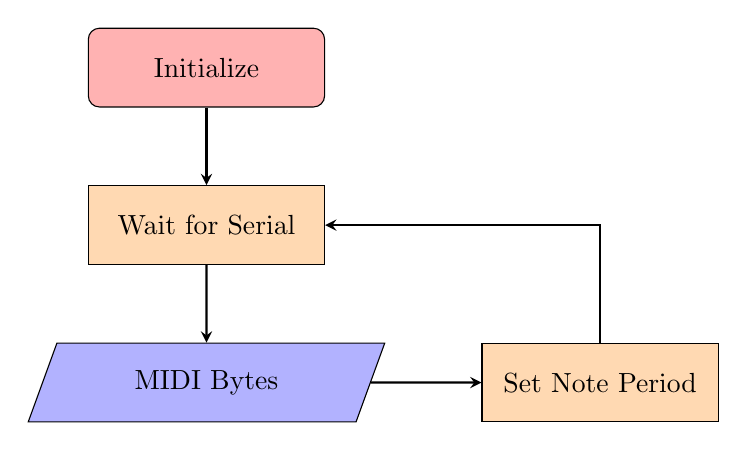
\begin{tikzpicture}[node distance=2cm]

\node (start) [startstop] {Initialize};
\node (process) [process, below of=start] {Wait for Serial};
\node (io) [io, below of=process] {MIDI Bytes};
\node (process1) [process, right of=io, xshift=3cm] {Set Note Period};


\draw [arrow] (start) -- (process);
\draw [arrow] (process) -- (io);
\draw [arrow] (io) -- (process1);
\draw [arrow] (process1) |- (process);

\end{tikzpicture}
\end{center}

This loop is represented in the loop function of the Arduino. This code is continuously waiting for serial data, and then it is parsed. The parsing follows the MIDI file format as discussed in Section \ref{MIDIMESSAGE}. The loop looks for note on, note off, zero velocity, and a channel mode message that occurs when the song ends. 

\lstinputlisting[language=C, firstline=95,lastline=121]{../src/floppy_uno/floppy_uno.ino}

\section{ISR}

The ISR or interrupt service routine is the routine that gets called every time the interrupt from the timer1 is triggered. The specific code run during this time is the code that does the driving of the floppy drives. The block diagram is as following:

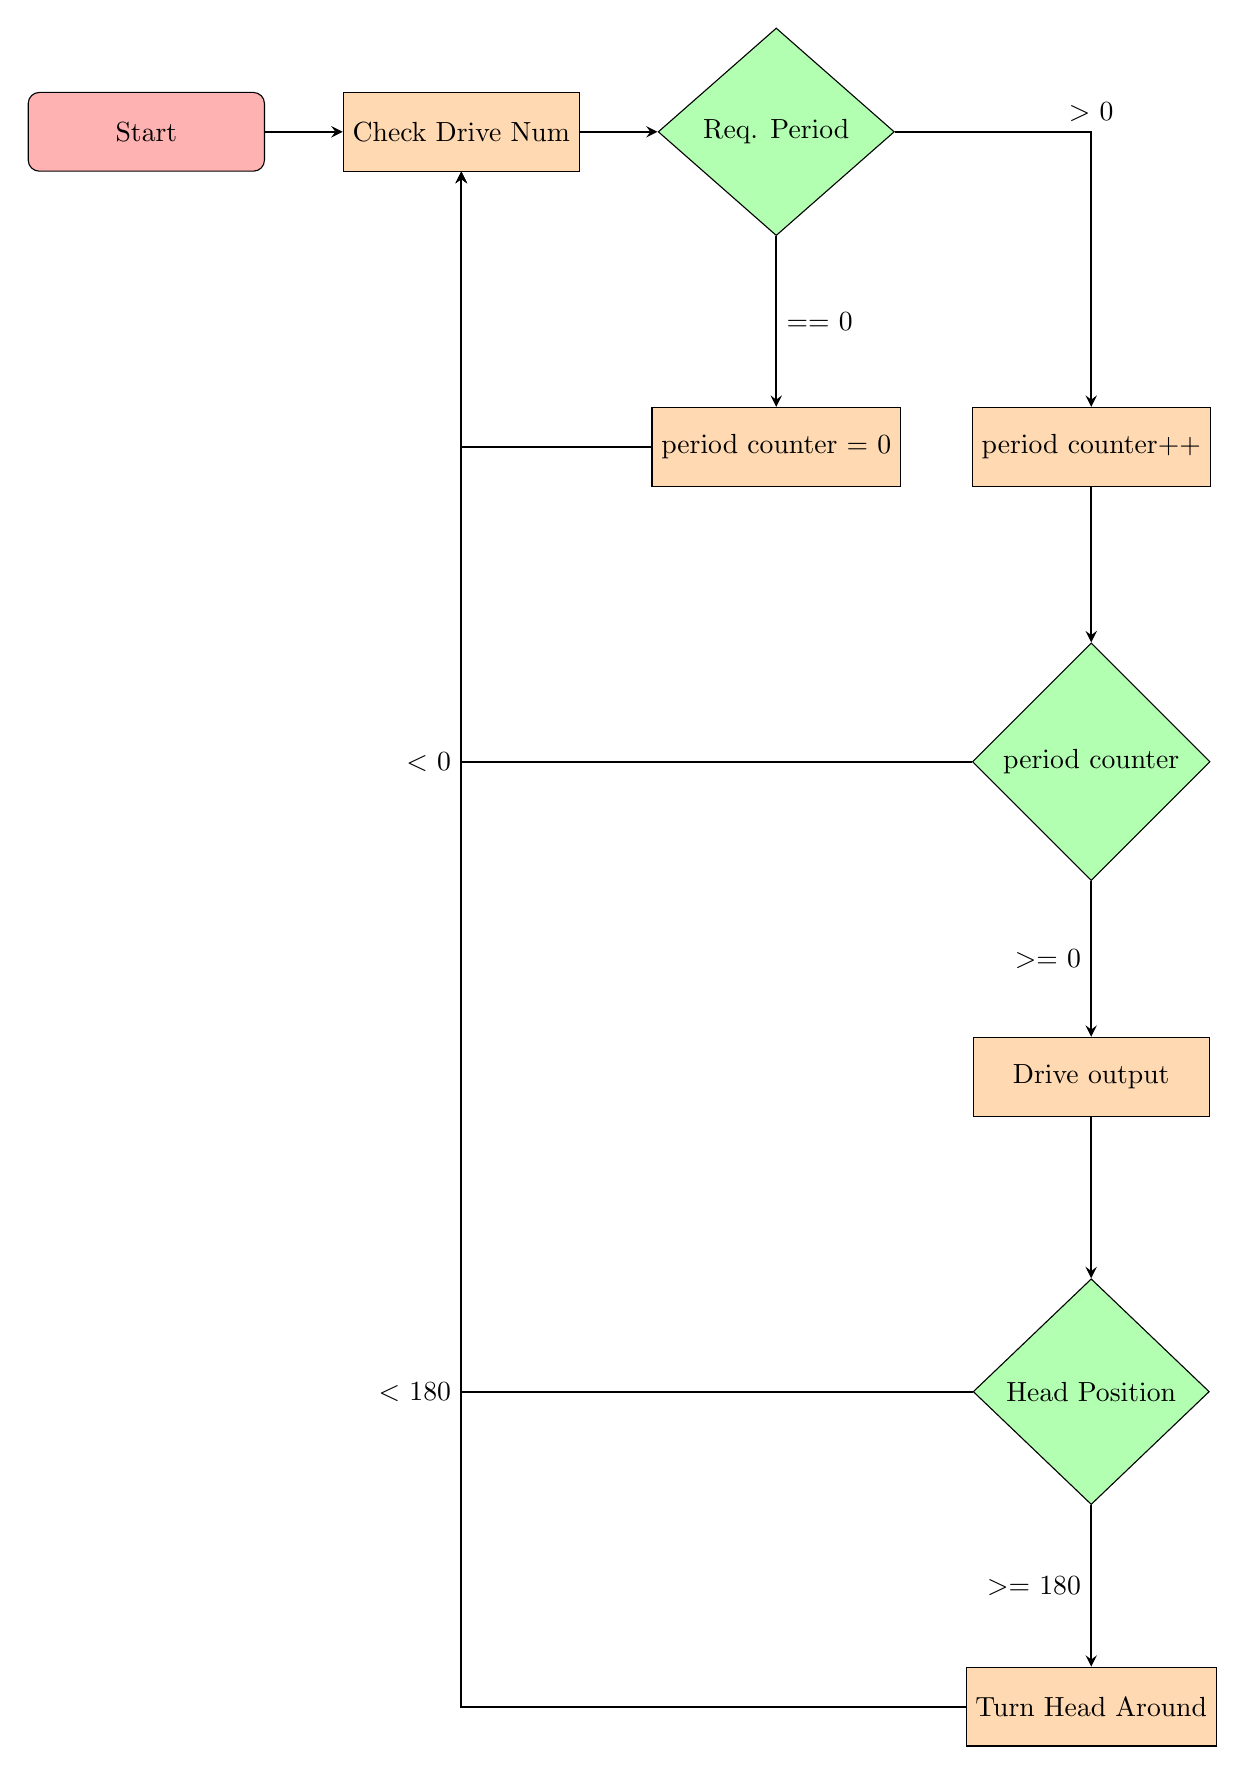
\begin{tikzpicture}[node distance=2cm]

\node (start) [startstop] {Start};
\node (process) [process, right of=start, xshift=2cm] {Check Drive Num};
\node (decision) [decision, right of=process, xshift=2cm] {Req. Period};
\node (process1) [process, below of=decision, yshift=-2cm] {period counter = 0};
\node (process2) [process, right of=process1, xshift=2cm] {period counter++};
\node (decision1) [decision, below of=process2, yshift=-2cm] {period counter};
\node (process3) [process, below of=decision1, yshift=-2cm] {Drive output};
\node (decision2) [decision, below of=process3, yshift=-2cm] {Head Position};
\node (process4) [process, below of=decision2, yshift=-2cm] {Turn Head Around};


\draw [arrow] (start) -- (process);
\draw [arrow] (process) -- (decision);
\draw [arrow] (decision) -- node[anchor=west] {== 0} (process1);
\draw [arrow] (decision) -| node[anchor=south] {$>$ 0} (process2);
\draw [arrow] (process1) -| (process);
\draw [arrow] (process2) -- (decision1);
\draw [arrow] (decision1) -| node[anchor=east] {$<$ 0} (process);
\draw [arrow] (decision1) -- node[anchor=east] {$>$= 0} (process3);
\draw [arrow] (process3) -- (decision2);
\draw [arrow] (decision2) -| node[anchor=east] {$<$ 180} (process);
\draw [arrow] (decision2) --  node[anchor=east] {$>=$ 180}  (process4);
\draw [arrow] (process4) -|(process);

\end{tikzpicture}

\pagebreak
The ISR follows a checklist. It is a for loop that checks each floppy drive's status. It first checks if notePeriod, or the requested period is greater than 0. If it is 0, that means that there is not a note assigned to that drive. Otherwise, it increments the period counter. If the period counter matches the notePeriod, it flips the step pin. This action of flipping will cause the read/write head to move every other time. It then resets the period counter so that it will start counting again. \\ 

The head position is also check to ensure that the read/write head does not get stuck at the ends of the track. If this variable has reached the maximum value, it will revert the direction by changing the value on the direction pin.

\lstinputlisting[language=C, firstline=122]{../src/floppy_uno/floppy_uno.ino}

\chapter{Future Work}

The floppy drive orchestra has room for a lot of improvement. As it is right now, the floppy drive orchestra successfully plays MIDI files that have been altered. There was an attempt to play any music and it demonstrated that even though the high notes cannot be played, the song can still be made out. The improvements to the orchestra fall under three main sections: transitioning it to an Arduino Mega, turning the Arduino into a MIDI player, and adjusting the bandwidth.\\

\section{Arduino Mega}
The first step is to transition the project over to an Arduino Mega. The Mega has a significant amount of digital pins that can be used to drive 16 floppy drives. Since the MIDI file format allows for 16 channels, it would be very useful to have 16 drives available so that any song can be played. \\

However, another system to make up for the lack of floppy drives is to build a system that dynamically allocates tasks to each floppy drive. Instead of directing the channels to one floppy drive at a time, the software would keep track of which drives were available. When a note on or off message for a channel is received, the software will look through all the drives to see if a drive is already servicing that channel. If so, the software will pass the message to that drive. Otherwise, it will pick a free drive and assign a channel to that drive. This method can reduce the number of drives necessary except for when a song utilizes all of the channels. \\

\section{Arduino as the MIDI Player}

The second step is to create a MIDI player on the Arduino itself by adding a microSD card and parsing through the MIDI files. This step is the most intensive step because the Arduino is replacing the MIDI player on the computer. This step eliminates the need of a computer, making the orchestra a plug and play. \\

The challenges with this step is to understand the MIDI file format and parse it through properly. Because of the different formats that MIDI has, it would require a very complex state machine be able to parse through it. Another issue is that depending on the format of the MIDI file, the different tracks are spread throughout the file. This means that the entire file must be parsed through before the entire song can be played. \\

The microSD card used can be found in Table \ref{fig:BOM}. The library is installed by default in Arduino under the header SD. There is a specific way the pins need to be connected. 

\captionof{table}{MicroSD Pinout to Arduino Mega}
\begin{center}
 \begin{tabular}{||c | c | c ||} 
 \hline
    Pin Name & MicroSD Pin & Arduino Mega Pin\\
 \hline
    Clock & Clk   & 52 \\
 \hline
    Chip Select & CS & 53 \\
 \hline 
    MOSI    & DO & 51 \\
 \hline
    MISO & DI & 50\\
    \hline
\end{tabular}
\end{center}

Once these are connect, it is greatly helpful to go through the SD header examples. An attempt to parse through a MIDI file is done in Appendix \ref{MEGACODE}.\\

In addition to using an SD card, the Arduino Timer3 library will be needed in order to properly act as a MIDI player. It is possible that more than Timer3 will be needed because different MIDI files may require more than one tempo. If that is the case, then each track will have to have its own timer to maintain the correct beat. \\

\section{Addressing the Bandwidth}

Because the floppy drive has a limited bandwidth, it would be difficult to be able to play any MIDI file that has not been altered. One method discussed would be to check the note and simply play the note, just an octave lower. This method is very simple, however, may cause the song to sound more dull.

\pagebreak

\appendix
\newappendix\label{UNOCODE}
\section{Arduino Uno Code}

\lstinputlisting[language=C]{../src/floppy_uno/floppy_uno.ino}


\newappendix\label{MEGACODE}
\section{Arduino Mega Code}

\lstinputlisting[language=C]{../src/floppy_mega/floppy_mega.ino}

\newappendix
\section{Bill of Materials}

\footnotesize{
\captionof{table}{Bills of Materials}\label{fig:BOM}
\begin{center}
 \begin{tabular}{|c | c | c | c |} 
 \hline
  \multicolumn{4}{|c|}{BOM} \\ 
 \hline
 ITEM & QUANTITY & COST & LINK \\
 \hline
 Arduino R3 & 1 & \$ 24.95 & \url{https://www.adafruit.com/product/50} \\
 \hline
 Arduino Proto Shield & 1 & \$ 9.95 & \url{https://www.adafruit.com/products/2077} \\
 \hline
 5V 4A Power Supply & 1 & \$ 14.95 & \url{https://www.adafruit.com/products/1466} \\
 \hline
 Breadboard-friendly 2.1mm DC barrel jack & 1 & \$ 0.95 & \url{https://www.adafruit.com/products/373} \\
 \hline
 (2.54mm) Crimp Connector Housing: 2x10-Pin & 2 & \$ 1.99 &  \url{https://www.pololu.com/product/1917} \\
 \hline
  (2.54mm) Crimp Connector Housing: 1x2-Pin & 2 & \$ 0.69 & \url{https://www.pololu.com/product/1901}\\
  \hline
  (2.54mm) Crimp Connector Housing: 2x2-Pin & 2 & \$ 0.59 & \url{https://www.pololu.com/product/1910}\\
 \hline
  (2.54 mm) Female Header: 1x12-Pin & 2 & \$ 0.79 & \url{https://www.pololu.com/product/1030}\\
  \hline
  (2.54 mm) Male Header: 2×40-Pin & 3 & \$ 1.49 & \url{https://www.pololu.com/product/966}\\
  \hline
   Pre-crimped Wires 10-Pack F-F (Black) & 4 & \$ 2.49 & \url{https://www.pololu.com/product/1810}\\
  \hline 
   Pre-crimped Wires 10-Pack F-F (Red) & 2 & \$ 2.49 & \url{https://www.pololu.com/product/1812}\\
  \hline 
   Pre-crimped Wires 10-Pack F-F (Blue) & 1 & \$ 2.49 & \url{https://www.pololu.com/product/1816}\\
  \hline 
   Pre-crimped Wires 10-Pack F-F (Purple) & 1 & \$ 2.49 & \url{https://www.pololu.com/product/1817}\\
  \hline
   MicroSD Breakout Board & 1 & \$ 7.50 & \url{https://www.adafruit.com/product/254}\\
  \hline
\end{tabular}
\end{center}
}

\renewcommand{\bibname}{References}
\begin{thebibliography}{9}
\bibitem{HairlessMIDI} Hairless MIDI Serial. 
\url{http://projectgus.github.io/hairless-midiserial/}
\bibitem{MIDIFileOutline}
MIDI File Structure. 
\url{http://www.ccarh.org/courses/253/handout/smf/} 
\bibitem{MIDIFormat}
Standard MIDI File Format.
\url{https://www.cs.cmu.edu/~music/cmsip/readings/Standard-MIDI-file-format-updated.pdf}
\bibitem{MIDIMessage}
Summary of MIDI Messages.
\url{https://www.midi.org/specifications/item/table-1-summary-of-midi-message}
\bibitem{MIDIStandard}
MIDI Tuning Standard. 
\url{https://en.wikipedia.org/wiki/MIDI_tuning_standard}
\bibitem{MIDITutorial}
MIDI Tutorial. 
\url{http://www.music-software-development.com/midi-tutorial.html}
\bibitem{Music}
Altered MIDI Music.
\url{https://github.com/coon42/Floppy-Music--midis-/tree/master/old}
\bibitem{pmidi}
Pmidi Source.
\url{http://alsa.opensrc.org/Pmidi}
\bibitem{ttymidi}
ttymidi Source.
\url{http://www.varal.org/ttymidi/}
\bibitem{VMPK}
VMPK Source.
\url{http://vmpk.sourceforge.net/}
\end{thebibliography}


\end{document}
